%!TEX TS-program = xelatex
%!TEX encoding = UTF-8 Unicode

\documentclass[10pt,a4paper]{article}

\setlength\topmargin{-48pt} % Top margin
\setlength\headheight{0pt} % Header height
\setlength\textwidth{7.0in} % Text width
\setlength\textheight{9.5in} % Text height
\setlength\oddsidemargin{-30pt} % Left margin
\setlength\evensidemargin{-30pt} % Left margin (even pages) - only relevant with 'twoside' article option

\usepackage{charter} % Charter font for main content

\frenchspacing % Reduces space after periods to make text more compact for a three-column layout

\usepackage{graphicx} % Required for including images
\usepackage{amssymb,amsmath} % Math packages
\usepackage{multicol} % Required for the three-column layout of the document
\usepackage{url} % Clickable links
\usepackage{enumitem} % Reduces the amount of space within and between lists with [noitemsep,nolistsep]
\usepackage{marvosym} % Required for the use of symbols
\usepackage{wrapfig} % Allows wrapping text around figures
\usepackage[T1]{fontenc} % Use 8-bit encoding that has 256 glyphs
\usepackage{datetime} % Required for defining a custom date style
\newdateformat{mydate}{\monthname[\THEMONTH] \THEYEAR} % Set a custom date format
\usepackage[pdfpagemode=FullScreen, colorlinks=false]{hyperref} % Link colors and PDF behavior in Acrobat
\usepackage{fancyhdr} % Required to define custom headers/footers
\pagestyle{fancy} % Enables the custom headers/footers for all pages following this

%% FONT SETTINGS --------------------------------------------------------
\usepackage{xeCJK}
\usepackage{fontspec,xltxtra,xunicode}% enable system font access
\defaultfontfeatures{Mapping=tex-text}
\setCJKmainfont{Hiragino Sans GB}
\setmainfont{Palatino Linotype}
\XeTeXlinebreaklocale “zh”
\XeTeXlinebreakskip = 0pt plus 1pt minus 0.1pt

% COLORFUL -----------------------------
%\usepackage[colorlinks=true]{hyperref}    % 生成帶書簽和超鏈接的PDF文件
\usepackage{color,xcolor}
\definecolor{hugored}{RGB}{232,83,104}
\definecolor{hugoyellow}{RGB}{255,200,104}
\definecolor{hugogreen}{RGB}{168,232,83}
\definecolor{hugocyan}{RGB}{102,255,238}
\definecolor{hugopurple}{RGB}{123,98,255}
\definecolor{hugoaqua}{RGB}{0,128,225}
\definecolor{hugostrawberry}{RGB}{225,0,128}
\definecolor{hugoteal}{RGB}{0,128,128}
% REFERENCE ------------------------------------------------------------
\usepackage{natbib}
\bibliographystyle{unsrt}

%-----------------------------------------------------------
% Header and footer
\lfoot{\footnotesize % Left footer containing newsletter contact information
雲加計算生物學和生物信息學通訊\\
%\Mundus\ \href{http://www.LaTeXTemplates.com}{LaTeXTemplates.com} \quad
\Telefon\ (028) 8657-0509 \quad
\Letter\ \href{mailto:huwung@gmail.com}{huwung.molnplus@gmail.com}
}

\cfoot{} % Empty center footer

\rfoot{\footnotesize ~\\ Page \thepage}

\renewcommand{\headrulewidth}{0.0pt} % No horizontal rule for the header
\renewcommand{\footrulewidth}{0.4pt} % Horizontal rule separating the footer from the document
%-----------------------------------------------------------

%-----------------------------------------------------------
% Define separators
\newcommand{\HorRule}[1]{\noindent\rule{\linewidth}{#1}} % Creates a horizontal rule
\newcommand{\SepRule}{\noindent	% Creates a shorter separator rule
\begin{center}
\rule{250pt}{1pt} % Page width and rule width
\end{center}
}
%-----------------------------------------------------------

%-----------------------------------------------------------
% Define title and article styles
\newcommand{\NewsletterName}[1]{ % Newsletter title
\begin{center}
\Huge \usefont{T1}{fvs}{b}{n} % Use the Bera Sans Bold font
#1
\end{center}	
\par \normalsize \normalfont}

\newcommand{\JournalIssue}[1]{ % Date and issue number at the top of the newsletter
\hfill \textsc{\mydate \today, No #1} % Right-aligned date and issue number
\par \normalsize \normalfont}

\newcommand{\NewsItem}[1]{ % News item title
\usefont{T1}{fvs}{n}{n} % Use the Bera Sans Normal font
\vspace{24pt}\large #1\vspace{3pt} % Print the title with space around it in a larger font size
\par \normalsize \normalfont}

\newcommand{\NewsAuthor}[1]{ % Author name under the item title
\hfill by \textsc{#1} \vspace{20pt} % Right-aligned author name in small caps with space after it
\par \normalfont}		

%----------------------------------------------------------------------------------------
%	TITLE
%----------------------------------------------------------------------------------------

\begin{document}

\JournalIssue{1} % Issue number

\NewsletterName{\small Newsletter of The {\color{hugostrawberry}{molN$+$}}\\ \huge 腫瘤與癌症} % Newsletter title

\noindent\HorRule{3pt} \\[-0.75\baselineskip] % Thick horizontal rule
\HorRule{1pt} % Thin horizontal rule

%----------------------------------------------------------------------------------------
%	MAIN NEWS ITEM
%----------------------------------------------------------------------------------------

\vspace{0.5cm}
\SepRule
\vspace{-0.5cm}

\begin{center}
\begin{minipage}[h]{0.75\linewidth}
\begin{wrapfigure}{l}{0.5\textwidth}

\includegraphics[width=0.42\textwidth]{molnplus.png}
\\
\end{wrapfigure}
	
\NewsItem{前言} % Main next item title
\vspace{3pt} % Some extra whitespace since there is no author as for the news in the body of the newsletter
\textit{
腫瘤或癌症依然是人類所面臨的最嚴重的健康負擔之一。
2014年6月发布的《2013年北京市卫生与人群健康状况报告》表明,2012年,北京市恶性肿瘤新发病例40307例,比上年增长了3.22\%。
这意味着2012年北京市平均每天有110人被确诊为癌症。而10年前,这一数字约为平均每天63人,相当于十年增长了将近一倍。
目前,先进的检测手段大大提高了确诊率。
繼而改善了早期癌症的治癒率。
}
\par\hfill --- molnplus
\end{minipage}
\end{center}

\vspace{0.5cm}
\SepRule % Small horizontal rule after the main news item
\vspace{0.5cm}

%\setlength{\columnsep}{16pt} % Uncomment to manually change the white space between columns
\begin{multicols}{2} % Begin the three-column layout

%----------------------------------------------------------------------------------------
%	OTHER NEWS
%----------------------------------------------------------------------------------------

\NewsItem{{\color{hugoteal}{The cancer glycocalyx mechanically primes integrin-mediated growth and survival}}}
\NewsAuthor{Matthew J. Paszek}

Malignancy is associated with altered expression of glycans and glycoproteins that contribute to the cellular glycocalyx.
We constructed a glycoprotein expression signature, which revealed that metastatic tumours upregulate expression of bulky glycoproteins.
A computational model predicted that these glycoproteins would influence transmembrane receptor spatial organization and function.
We tested this prediction by investigating whether bulky glycoproteins in the glycocalyx promote a tumour phenotype in human cells by increasing integrin adhesion and signalling.
Our data revealed that a bulky glycocalyx facilitates integrin clustering by funnelling active integrins into adhesions and altering integrin state by applying tension to matrix-bound integrins, independent of actomyosin contractility.
Expression of large tumour-associated glycoproteins in non-transformed mammary cells promoted focal adhesion assembly and facilitated integrin-dependent growth factor signalling to support cell growth and survival.
Clinical studies revealed that large glycoproteins are abundantly expressed on circulating tumour cells from patients with advanced disease.
Thus, a bulky glycocalyx is a feature of tumour cells that could foster metastasis by mechanically enhancing cell-surface receptor function.\cite{PasDuFRos1406}

%-----------------------------------------------------------

\NewsItem{{\color{hugored}{Cancer: Sugar-coated cell signalling}}}
\NewsAuthor{Andrew J. Ewald and Mikala Egeblad}

Cell membranes are covered with sugar-conjugated proteins.
New findings suggest that the physical properties of this coating, which is more pronounced in cancer cells, regulate cell survival during tumour spread.\cite{EwaEge1406}

%-----------------------------------------------------------

\begin{quotation} % Example of a quotation
\noindent{\Huge``}

\noindent\normalsize\textit{[肿瘤细胞的保护层] 细胞糖萼 (覆盖细胞表面的一个糖蛋白/多糖层) 的组成通过组织分化和疾病等过程随细胞性质的变化而变化。
Valerie Weaver及同事试图弄清癌细胞中糖萼组成的变化是否会影响癌症表现型。
他们发现,大块糖萼是转移性癌细胞的一个特征,是由大型糖蛋白的生成而产生的。
大块糖萼会以物理方式将被称为``整联蛋白''或``粘合素''的糖蛋白粘附分子束缚住,后者反过来又会促进一个有利于细胞生存和增殖的信号传导体系。
临床研究显示,大型糖蛋白在来自侵袭性乳腺癌患者的循环肿瘤细胞上大量表达。
这些发现表明,糖萼及其分子组分是以使跨膜受体信号传导正常化为目的的治疗干预的有吸引力的目标。\cite{PasDuFRos1406,EwaEge1406}}

\hfill{\Huge''}

\hfill-- molnplus
\end{quotation}

% -----------------------------------

\end{multicols} % End the three-column layout for a large picture

\begin{center}
\vspace{10pt}

\includegraphics[width=1\linewidth]{cancer-fight-blogs.jpg} % Example of an image taking up the total width of the page
\par\large\textit{http://blogs.independent.co.uk\ldots}
\vspace{10pt}
\end{center}

\begin{multicols}{2}

\NewsItem{BRCA2 prevents R-loop accumulation and associates with TREX-2 mRNA export factor PCID2}
\NewsAuthor{Vaibhav Bhatia}

Genome instability is central to ageing, cancer and other diseases. It is not only proteins involved in DNA replication or the DNA damage response (DDR) that are important for maintaining genome integrity: from yeast to higher eukaryotes, mutations in genes involved in pre-mRNA splicing and in the biogenesis and export of messenger ribonucleoprotein (mRNP) also induce DNA damage and genome instability. This instability is frequently mediated by R-loops formed by DNA-RNA hybrids and a displaced single-stranded DNA. Here we show that the human TREX-2 complex, which is involved in mRNP biogenesis and export, prevents genome instability as determined by the accumulation of γ-H2AX (Ser-139 phosphorylated histone H2AX) and 53BP1 foci and single-cell electrophoresis in cells depleted of the TREX-2 subunits PCID2, GANP and DSS1. We show that the BRCA2 repair factor, which binds to DSS1, also associates with PCID2 in the cell. The use of an enhanced green fluorescent protein-tagged hybrid-binding domain of RNase H1 and the S9.6 antibody did not detect R-loops in TREX-2-depleted cells, but did detect the accumulation of R-loops in BRCA2-depleted cells. The results indicate that R-loops are frequently formed in cells and that BRCA2 is required for their processing. This link between BRCA2 and RNA-mediated genome instability indicates that R-loops may be a chief source of replication stress and cancer-associated instability.\cite{BhaBarGar1406}

\begin{quotation} % Example of a quotation
\noindent{\Huge``}

\noindent\normalsize\textit{[利用R-环来促进癌症] R-环(自然出现的三链核酸结构,由一个RNA–DNA杂合体和被取代的单链DNA组成)是基因组不稳定性的潜在诱导因素之一。
这项研究显示,TREX-2 (在“信使核糖核蛋白”(mRNP)的生物生成和输出中所涉及的一种复合物)通过与乳腺癌易感基因因子 BRCA2相互作用来处理R-环。
不含BRCA2的人细胞会积累高水平的R-环。
在肿瘤抑制因子与R-环之间的这一出乎意料的相互作用表明,R-环也许是造成复制应激和肿瘤发生的一个主要原因。}

\hfill{\Huge''}

\hfill-- molnplus
\end{quotation}

%-----------------------------------------------------------

\NewsItem{{\color{hugoteal}{Notch-Dependent Repression of miR-155 in the Bone Marrow Niche Regulates Hematopoiesis in an NF-$\kappa$B-Dependent Manner}}}
\NewsAuthor{Wang Lin}

The microRNA miR-155 has been implicated in regulating inflammatory responses and tumorigenesis, but its precise role in linking inflammation and cancer has remained elusive.
Here, we identify a connection between miR-155 and Notch signaling in this context.
Loss of Notch signaling in the bone marrow (BM) niche alters hematopoietic homeostasis and leads to lethal myeloproliferative-like disease.
Mechanistically, Notch signaling represses miR-155 expression by promoting binding of RBPJ to the miR-155 promoter.
Loss of Notch/RBPJ signaling upregulates miR-155 in BM endothelial cells, leading to miR-155-mediated targeting of the nuclear factor $\kappa$B (NF-$\kappa$B) inhibitor $\kappa$B-Ras1, NF-$\kappa$B activation, and increased proinflammatory cytokine production.
Deletion of miR-155 in the stroma of RBPJ(-/-) mice prevented the development of myeloproliferative-like disease and cytokine induction.
Analysis of BM from patients carrying myeloproliferative neoplasia also revealed elevated expression of miR-155.
Thus, the Notch/miR-155/$\kappa$B-Ras1/NF-$\kappa$B axis regulates the inflammatory state of the BM niche and affects the development of myeloproliferative disorders.\cite{wang2014notch}

% ---------------------

\begin{center}
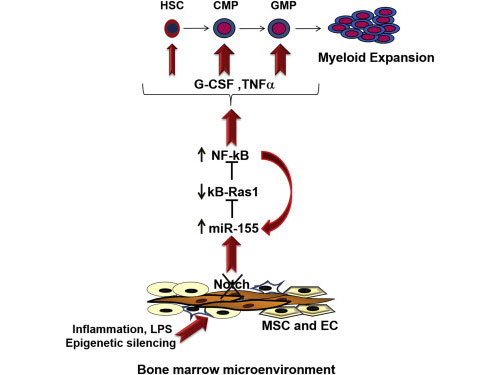
\includegraphics[width=0.8\linewidth]{microenvironment.png} % Example of an in-line image
\end{center}

%-----------------------------------------------------------


\begin{quotation}
\noindent{\Huge``}

\noindent\normalsize\textit{[炎症和癌症关系]由印第安纳大学儿科副教授Nadia Carlesso博士领衔的研究团队发现,类似一串倒下的多米诺骨牌一样,骨髓中的一连串分子事件会产生高水平的炎症反应,该反应会扰乱正常的血液形成,从而可能会导致白血病。这项研究的成果7月3日发表在Cell Stem Cell杂志上。该研究指出了一条可能的治疗血液病的新策略,进一步阐明了炎症和癌症之间的关系。\\
骨髓中包含造血过程产生的白血球和红血球,而骨髓同时也为造血细胞提供了支持系统(被称作造血微环境)。最新的研究提示了造血微环境在一系列潜在致命疾病(被称作骨髓增生性疾病)的进程中起到的重要作用。实际上,多年来人们已经知道炎症和癌症之间的联系。例如,已知骨髓中的高水平炎症和骨髓增生性疾病的发展相关,而骨髓增生性疾病会因为产生过多的髓细胞(这些细胞正常情况下用来抵御感染)导致严重的疾病。这些疾病给患者带来心脏病发作和中风的危险,并常发展为急性白血病和骨髓衰竭。而目前这些研究缺乏基因模型,特别是对于血液相关的恶性肿瘤,尚没有有效的疗法治疗大部分骨髓增生性疾病。\\
此次研究针对在血细胞产生的过程中起到重要作用的Notch分子发生异常而导致表达水平降低的现象,研究人员使用基因修饰的小鼠发现,造血微环境中如果缺失Notch会引发一连串的分子事件,结果产生一连串的炎症因子。研究人员阻断了这个生化级联反应链中的一个分子的活动后,小鼠上的骨髓增生性疾病发生了逆转。此外,人类骨髓增生性疾病患者体内该分子的水平也有明显提高。这些发现提示,针对这个免疫反应过程中的不同关键点来开发药物可能是个有潜力的治疗骨髓增生性疾病的策略。Carlesso表示此次研究的另一关键发现是,引起炎症反应的分子链并不直接发生在骨髓造血细胞中,而是存在于构成骨髓微环境的细胞中,特别是在内皮细胞中。\\
这项工作提示人们不仅需要靶向肿瘤细胞,还应当靶向环绕肿瘤细胞的炎症微环境中的细胞。研究人员相信该策略会在阻止骨髓增生性疾病的进展和急性白血病转移中展现疗效。Carlesso博士还指出Notch分子大多被称为原癌基因,因此过去的研究往往都是靶向Notch基因治疗。该研究提示医生们需要意识到降低Notch功能水平能够抑制血液病发展进程。}


\hfill{\Huge''}

\hfill-- molnplus
\end{quotation}

%\end{multicols}
%-----------------------------------------------------------

\NewsItem{{\color{hugored}{討論與總結}}}
据统计,我国每年新患癌症的病人约160万人,每年因癌症死亡的人数约130万人。
我国大、中城市居民的许多死亡原因中,癌症是第一位死因,在农村的各项死因中,癌症是第二位死因。
对中、老年人来说癌症是多发病、常见病。
对早期癌症病人的治疗约有80\%-90\%以上可以治愈;
但是,晚期的癌症病人,在治疗后能生存5年以上的人,就比较少了。
早期癌症病人治疗后,不仅提高了生存率,同时也提高了病人的生存质量。
癌症病人的死亡率随之也降下来了。
众所周知,早期癌症病人的治疗要比晚期癌症病人的治疗节省许多人力、财力和时间。
所以我们提倡癌症病人要早期发现、早期诊断、早期治疗。
在有条件的地方,定期开展健康检查或防癌普查(初筛)对发现早期癌症是较好的方法。

本期回顧了近來癌症基礎研究和臨床干預的進展。

腫瘤細胞的保護層可能是耐藥性產生的原因之一。

三鏈核酸結構是基因組不穩定性產生的重要原因之一,繼而導致複製應激和腫瘤發生。
這或許能成為癌症早期診斷的新的臨床指標。
相對于免疫檢測法,核酸的檢測更為準確快速。
(怎麼檢測血樣中的三鏈核酸結構是我們團隊所面臨的最大問題)

早期诊断是指在患者出现临床症状前或在癌症发生浸润前得以确诊,繼而進行及时有效地干預,籍此达到改善预后,减轻患者痛苦和精神和经济负担,提高治愈率,以及降低死亡的目的。

超早期检测是腫瘤篩查的重要方法。
蛋白质指纹图谱 (蛋白指纹法) 分析诊断的发展将是分子医学领域的一场革命,它不仅提供了一种新的检测方法,并且具有很高的可行性。
它可在数分钟时间内从微量血液中测出上千个结果并对其进行分析。
美国NCI (National Cancer Institute) 主席 Dr. Andrew von Eschenbach在2005年4月16日 (美国第96届肿瘤年会上) 宣布美国将用蛋白指纹图谱技术对肿瘤早期定性和PET-CT对肿瘤早期定位相结合的等手段对肿瘤做出极早期诊断,使肿瘤在2015年成为非致死性疾病。


% ------------------------------------------
\begin{center}

\includegraphics[width=1\linewidth]{molnplus.png} % Example of an in-line image
\end{center}

\end{multicols}

% ---------------------------
% \begin{multicols}{2}

\begin{center}

\noindent\HorRule{3pt} \\[-0.75\baselineskip] % Thick horizontal rule
\HorRule{1pt} % Thin horizontal rule
% \rule{500pt}{1pt} % Page width and rule width

參與該工作的團隊成員:
王虎
\end{center}

% \end{multicols}
%----------------------------------------------------------------------------------------
\newpage

\bibliographystyle{unsrt}
\bibliography{/Users/wanghu/phenomenon/personlig/references/molnplus}

\end{document} 
